\documentclass[conference]{IEEEtran}
\IEEEoverridecommandlockouts
\usepackage{cite}
\usepackage{amsmath,amssymb}
\usepackage{graphicx}
\usepackage{booktabs}
\usepackage{multirow}
\usepackage{xcolor}
\usepackage{url}
\usepackage[hidelinks]{hyperref}
\graphicspath{{figs/}}

\newcommand{\cond}[1]{\textsc{#1}}

\begin{document}

\title{Talk or Map? What Should Robot Teams Share?}

\author{\IEEEauthorblockN{Siddharth Choudhary}
\IEEEauthorblockA{\url{https://itzsid.github.io/hivemap/}}}

\maketitle

\begin{abstract}
When every robot in a team runs its own language-model agent, the team needs a way to pool what its members have seen.
Multi-robot LLM systems usually let the robots talk to each other in natural language, while collaborative SLAM systems fuse what the robots have seen into one map.
We ask which of the two a team should share, and when.
We built Hivemap, an open-source testbed that runs in a web browser.
In it, up to ten simulated robots with drifting odometry and open-vocabulary object detections explore six buildings, then carry out five kinds of task: go to an object, count a category, meet at a landmark, visit every instance of a category, and find a lost item.
The robots either work alone, exchange short natural-language messages, or merge their object maps through verified cross-robot data association and distributed pose-graph optimization.
Across 3{,}582 simulated episodes, language messages make fetch, rendezvous, and search two to three times faster than working alone for under 1\,kB, but no more reliable, because the robot that hears a description must find and recognize the object itself.
The verified, optimized map makes fetch and rendezvous seven to ten times faster than working alone and succeeds in 96--98\% of those episodes, within two points of a ground-truth map.
It costs about 400\,kB per episode, roughly 600 times the messages.
Talking is enough for counting a category and for covering it room by room.
A map that is merged but not optimized, or merged from unchecked object matches, is less reliable than no sharing at all on several tasks.
The whole system, including in-browser language-model agents that choose among these same tools, runs on a laptop.
\end{abstract}

%% =====================================================================
\section{Introduction}\label{sec:intro}

Picture ten robots that have spent the night patrolling a hospital wing.
Each one has seen a different part of the building.
In the morning a nurse asks one of them to fetch the wheelchair from Room~203, a room that robot has never entered.
Somebody on the team has seen that wheelchair.
How should that knowledge reach the robot that needs it?

Two research communities have given two different answers.
Work on large language models (LLMs) for multi-robot teams gives each robot an agent and lets the agents \emph{talk}: they negotiate plans~\cite{mandi2024roco}, decide what to tell their teammates~\cite{zhang2024coela}, or route messages through a central or hierarchical planner~\cite{chen2024scalable,kannan2024smartllm}.
Work on collaborative SLAM instead fuses the robots' observations into a single consistent \emph{map}~\cite{choudhary2017ijrr,tian2022kimeramulti,lajoie2024swarmslam}, increasingly with open-vocabulary object labels that a language model can query~\cite{chang2023hydramulti,gu2025mrcographs}.
Each community tends to assume its own medium.
LLM-team papers rarely build a map, and when LLM planners do use a shared map, the map is usually assumed to be correct, with known robot poses~\cite{yu2023conavgpt,shen2025mcoconav,wang2025comresvlm}.
Collaborative SLAM papers measure trajectory error and bandwidth, not whether the map helps a team finish a job.

This paper puts the two media side by side.
We hold the buildings, robots, tasks, and decision rules fixed and change only what the robots share:
\begin{itemize}
\item \cond{Alone}: nothing; each robot uses only what it saw itself.
\item \cond{Language}: short natural-language messages that name objects and rooms, as a language agent would write them.
\item \cond{Map}: an object map merged across robots, built under unknown initial frames, verified against perceptual aliasing, and either used as merged or refined by distributed pose-graph optimization~\cite{choudhary2016icra,choudhary2017ijrr}.
\end{itemize}
The map is not handed to the robots.
They build it from noisy odometry and detections, find each other's frames by meeting or by matching objects, and pay for it in bandwidth.
Merging errors, rejected look-alike matches, and residual drift are therefore part of what we measure.

Our contributions are:
\begin{enumerate}
\item \textbf{Hivemap}, an open-source multi-robot testbed that runs in the browser, with up to ten robots, six buildings (including a hospital wing with ten look-alike patient rooms), five task families, and per-robot LLM agents that call mapping and messaging operations as tools (Fig.~\ref{fig:teaser}).
\item A \textbf{controlled comparison} of the three media over 3{,}582 episodes, reporting success, completion time, distance driven, and bytes sent per channel.
\item \textbf{Findings} on when each medium is enough. Words tell a robot where to look; a verified map tells it where to go and which object is meant. The map pays off only when it is optimized and its merges are checked.
\end{enumerate}

We do not propose a new SLAM back-end or a new LLM planner.
The two-stage distributed solver is from our earlier work~\cite{choudhary2016icra,choudhary2017ijrr}, the verification rules follow established practice for robust inter-robot loop closures~\cite{mangelson2018pcm,yang2020gnc}, and the agents follow the familiar tool-calling pattern~\cite{yao2023react}.
What is new is the question and the measurement.

\begin{figure*}[t]
\centering
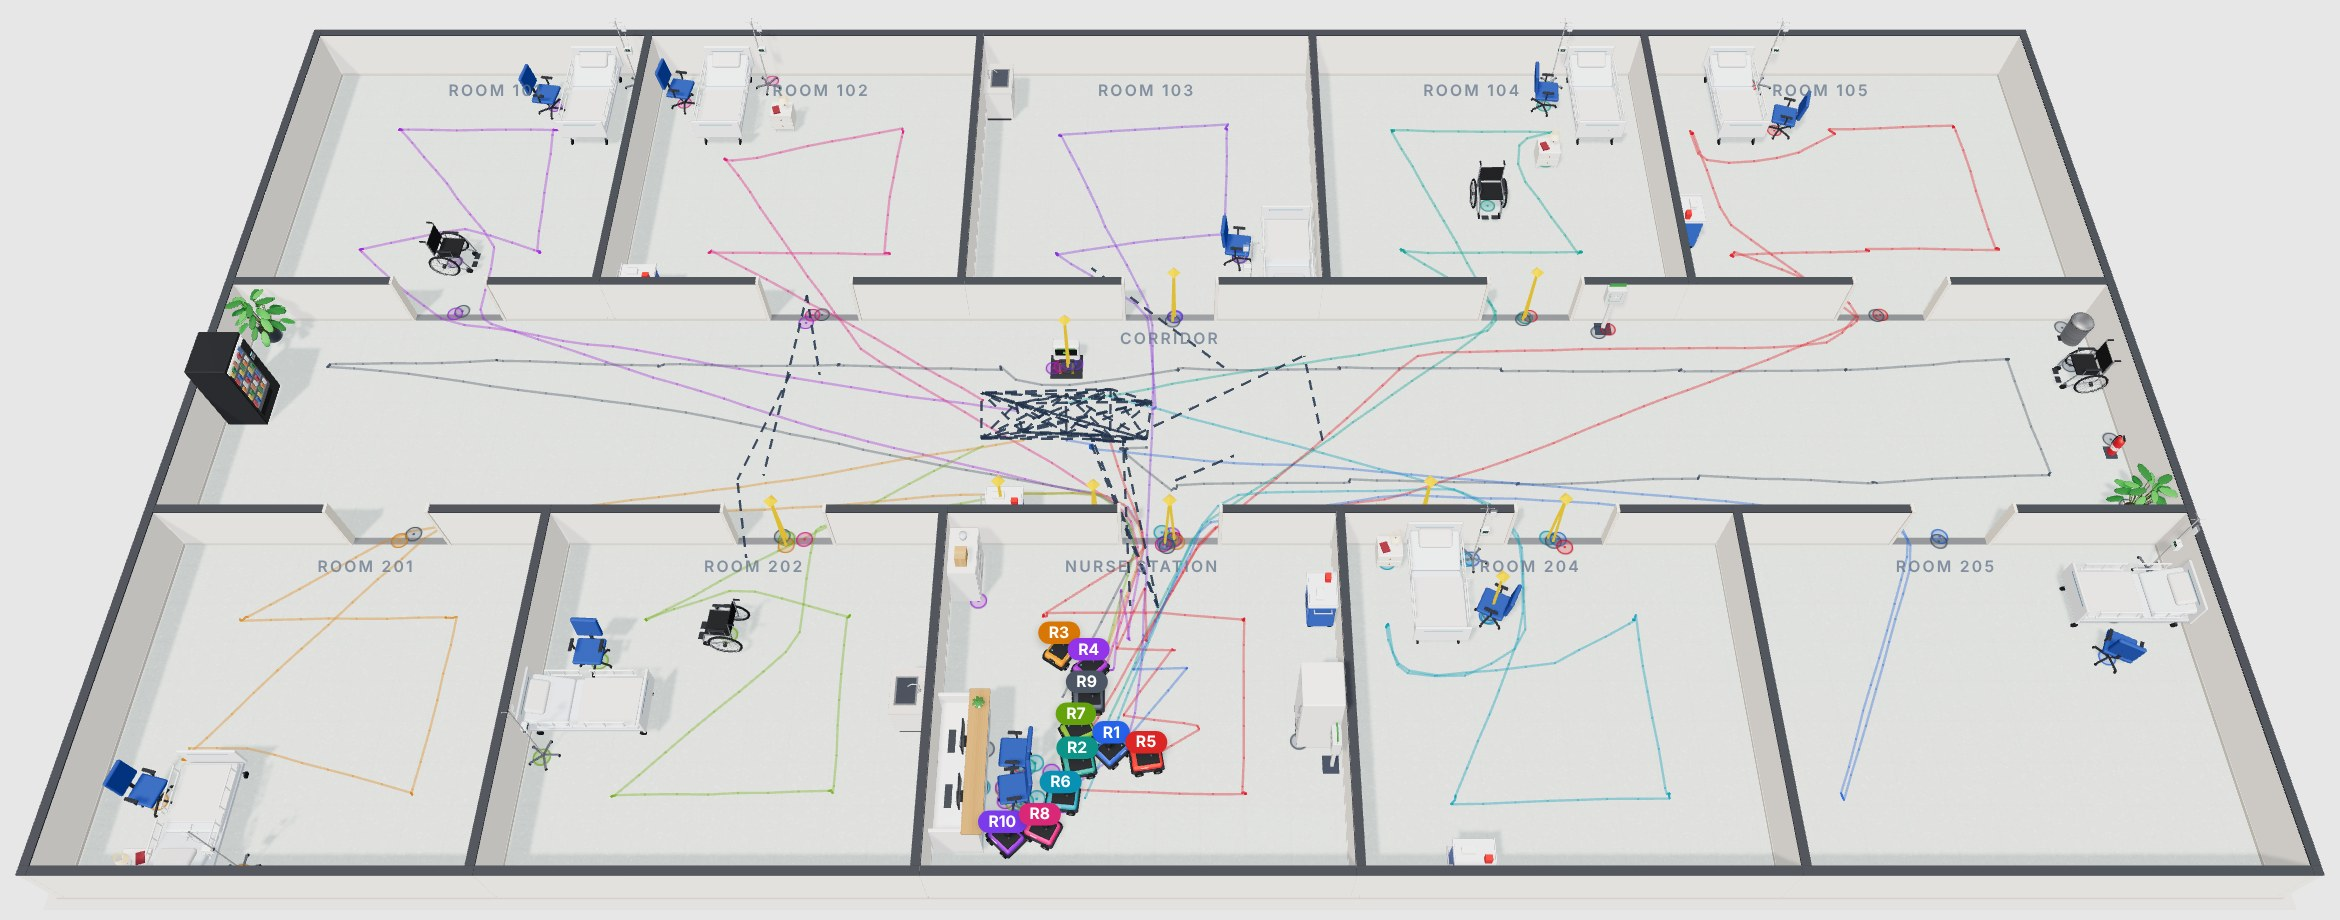
\includegraphics[width=\textwidth]{teaser.jpg}
\caption{\textbf{Hivemap.} Ten robots in a simulated hospital wing after the instruction ``Explore the building.'' Each colored line is one robot's path. Gold markers are objects that two or more robots saw; once verified, they tie the robots' maps together. The robots then meet at the nurse station using the merged map. The live demo at \url{https://itzsid.github.io/hivemap/} runs this simulation, the map merging, and one language-model agent per robot in the browser.}
\label{fig:teaser}
\end{figure*}

%% =====================================================================
\section{Related Work}\label{sec:related}

\textbf{Collaborative SLAM.}
Distributed and decentralized multi-robot SLAM has a long history.
It includes distributed smoothing~\cite{cunningham2010ddfsam}, two-stage distributed Gauss-Seidel estimation with object-based landmarks~\cite{choudhary2016icra,choudhary2017ijrr}, data-efficient decentralized visual SLAM~\cite{cieslewski2018icra}, and certifiably correct distributed pose-graph optimization~\cite{tian2021dc2pgo}.
Complete systems include DOOR-SLAM~\cite{lajoie2020doorslam}, Kimera-Multi~\cite{chang2021kimeramulti,tian2022kimeramulti}, Swarm-SLAM~\cite{lajoie2024swarmslam}, COVINS~\cite{schmuck2021covins}, and the field-tested LAMP~\cite{ebadi2020lamp,chang2022lamp2}; see~\cite{lajoie2022survey} for a survey.
A wrong inter-robot loop closure can corrupt the whole map, so pairwise consistency maximization~\cite{mangelson2018pcm} and graduated non-convexity~\cite{yang2020gnc} are now standard.
When the robots' initial frames are unknown, maps can be merged from direct robot-robot observations~\cite{zhou2006rendezvous,howard2006ijrr}.
Hivemap reuses these ideas.
These systems are evaluated by trajectory and map accuracy; we evaluate the map by what it lets a team of agents do, and against a language baseline.

\textbf{Open-vocabulary object maps and scene graphs.}
Object-level SLAM~\cite{salasmoreno2013slampp,nicholson2019quadricslam,yang2019cubeslam} and foundation-model features~\cite{radford2021clip,kirillov2023sam,ravi2025sam2} have produced maps that can be queried in words, including dense feature fields~\cite{peng2023openscene,jatavallabhula2023conceptfusion} and object graphs~\cite{gu2024conceptgraphs,werby2024hovsg,maggio2024clio}.
Multi-robot versions build and share 3D scene graphs~\cite{chang2023hydramulti}, compress them for transmission~\cite{chang2023dlite}, or share open-vocabulary object graphs at a fraction of the bandwidth~\cite{gu2025mrcographs}.
These are more capable map builders than ours, which uses simulated stand-in features (Sec.~\ref{sec:limits}).
They do not put language agents in the loop, and they do not compare map sharing with talking.

\textbf{LLM agents for multi-robot teams.}
LLMs plan for single robots by grounding language in affordances~\cite{ahn2022saycan}, code~\cite{liang2023cap}, feedback~\cite{huang2022innermonologue}, or a given 3D scene graph~\cite{rana2023sayplan}.
For teams, RoCo~\cite{mandi2024roco} has per-robot LLMs negotiate in dialogue, SMART-LLM~\cite{kannan2024smartllm} decomposes and allocates tasks centrally, and Chen et al.~\cite{chen2024scalable} compare centralized, decentralized, and hybrid dialogue structures as the team grows.
CoELA~\cite{zhang2024coela} builds embodied agents that decide what to say to each other and finds that language helps, but that many LLM messages are redundant.
A second line gives an LLM or VLM planner a shared semantic map for multi-robot search and navigation~\cite{yu2023conavgpt,shen2025mcoconav,wang2025comresvlm}; there the map is typically fused centrally under known poses.
Murata et al.~\cite{murata2025multiobject} plan multi-object retrieval with knowledge distributed across robots.
Prior work therefore fixes the medium, either language or a trusted map.
We vary it while holding everything else fixed, and we include the cost and errors of building the map.

\textbf{Task allocation.}
Our dispatcher is a classical cost-based allocator~\cite{gerkey2004taxonomy,dias2006market}, and our room-splitting search is a simple form of coordinated exploration~\cite{burgard2005coordinated}.
We claim nothing new here.
The point is that path-cost allocation needs metric positions in a common frame, which language replies do not provide.

%% =====================================================================
\section{Hivemap}\label{sec:method}

Fig.~\ref{fig:pipeline} shows the pipeline.
Each robot builds its own object map.
When asked, the team exchanges maps, finds each robot's frame relative to the others, verifies which objects are shared, and optionally optimizes the joint pose graph.
Agents or scripted policies then act on the result.
Everything runs in JavaScript in the browser and, for experiments, headless in Node.js with a fixed random seed.

\begin{figure*}[t]
\centering
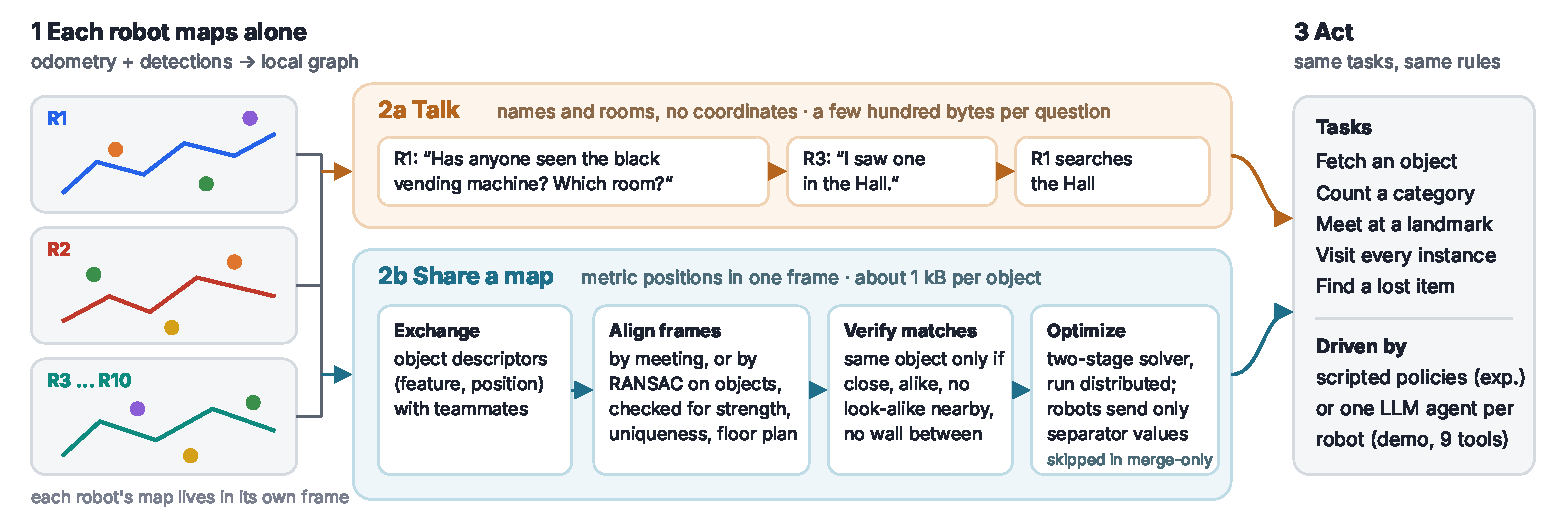
\includegraphics[width=0.92\textwidth]{pipeline.pdf}
\caption{\textbf{Pipeline.} Each robot runs local object SLAM. In the \cond{Map} conditions, robots exchange compact object descriptors, align their frames by meeting each other or by matching objects, verify which objects are the same physical thing, and solve the joint pose graph with the two-stage distributed solver. In \cond{Language}, robots instead answer questions in words from their own maps.}
\label{fig:pipeline}
\end{figure*}

\subsection{Buildings, robots, and sensing}
Six floor plans cover common indoor settings: an office (24\,m$\times$16\,m, 5 rooms), a warehouse with occluding racks and many identical pallets (36$\times$22\,m, 3 areas), an apartment (20$\times$14\,m, 5 rooms), a hospital wing with ten nearly identical patient rooms off one corridor (36$\times$18\,m, 11 rooms), a retail store with shelf aisles (30$\times$20\,m, 4 areas), and a lab building (32$\times$18\,m, 7 rooms).
They contain 33 to 65 objects each, from 51 categories in nine colors.
Robots are differential-drive bases (0.56$\times$0.44\,m, up to 1\,m/s) that plan on an occupancy grid, follow smoothed paths, and yield to each other.
They record a keyframe every 0.5\,m or 30$^\circ$.
Odometry has 3.5\% translational and 1.5\% rotational noise per step, a per-robot gyro bias of up to 0.014\,rad/m, and occasional wheel slip.
The camera has a 90$^\circ$ field of view.
An object at range $r$ is detected with probability $0.97\,(1-(r/R)^3)$, where $R$ is 2.6\,m for small objects, 6\,m for large ones, and 5\,m otherwise.
Walls and tall furniture block the view, 2\% of detections are false, and an object enters a robot's map only after two sightings.

\textbf{Open-vocabulary features.}
We do not render images.
Each detection carries a 48-dimensional unit descriptor that mixes a fixed direction for its category with a weaker direction for its color, plus view noise.
Text queries such as ``orange armchair'' embed into the same space.
This stands in for mask-plus-CLIP features~\cite{ravi2025sam2,radford2021clip}.
It reproduces the property that matters here, that objects of the same kind and color look alike, but it is cleaner than real features.

\subsection{Local object SLAM}
Each robot keeps a pose graph of its keyframes and the objects it has seen, with odometry factors between consecutive keyframes and relative-pose factors from keyframes to objects.
We solve it with the two-stage method of~\cite{choudhary2016icra}: first rotations, as a linear least-squares problem over unit complex numbers, then translations given the rotations.
Both stages use Gauss-Seidel sweeps with successive over-relaxation ($\omega=1.9$) and warm starts.

\subsection{Merging maps under unknown frames}\label{sec:merge}
Robots start from a common dock but do not know their relative poses.
Each robot's map is expressed in its own starting frame.
To merge maps, robots exchange object descriptors, and the team adds robots one at a time to a growing joint map.
We count 1{,}040 bytes per object sent, as if each descriptor carried a 512-dimensional half-precision CLIP feature plus its position and id.

\textbf{Frame alignment.}
If two robots have met (within 4\,m with a clear line of sight), the measured relative pose aligns their frames directly, in the spirit of~\cite{zhou2006rendezvous,howard2006ijrr}.
Otherwise we propose candidate object matches by descriptor similarity (cosine $>0.8$) and fit a 2D rigid transform with two-point RANSAC.
Look-alike rooms make this risky: in the hospital, five patient rooms each hold a bed, a chair, and an IV stand in the same arrangement.
We therefore accept an alignment only if it passes three checks.
(i)~\emph{Strength}: at least five inliers from at least three categories, or four inliers from two categories with residual below 0.3\,m spread over more than 2.5\,m.
(ii)~\emph{Uniqueness}: no rival hypothesis that places the map more than 1.2\,m or 0.3\,rad away has more than 60\% of the inliers or comes within two inliers of the best.
(iii)~\emph{Floor-plan consistency}: once aligned, no more than 2\% of the robot's trajectory may pass through a wall.
We assume the floor plan is known, as it usually is for facility robots.

\textbf{Object association.}
Given the frames, two objects from different robots become one shared object if they are within 1\,m, their descriptors agree, they are not on opposite sides of a wall, and neither robot has a look-alike within a radius $A=\max(1.5,\,2.5(\sigma_a+\sigma_b))$\,m.
Here $\sigma = 0.1 + 0.04\,d$ grows with the distance $d$ the robot had driven before first seeing the object, so the gate widens with accumulated drift.
Each accepted match adds a ``same object'' factor between the two robots' landmarks, and each meeting adds a relative-pose factor between their keyframes.

\textbf{Placing maps in the floor plan.}
Robots navigate on the known floor plan, so a map must be placed in it.
A real robot would do this by localizing against the floor plan.
In simulation we take a shortcut: we place each robot's own map, and the merged team map as a whole, with a least-squares rigid fit of the estimated trajectory to the true one.
This removes the global offset but keeps the map's internal distortion, including any distortion that a wrong merge causes.
It applies equally to every condition, including \cond{Alone} and \cond{Language}, and it makes absolute position errors optimistic (Sec.~\ref{sec:limits}).

\subsection{Distributed optimization}
The joint graph is solved with the same two-stage solver run in its distributed form~\cite{choudhary2016icra,choudhary2017ijrr}.
Each robot updates only its own poses and landmarks and, after every round, sends its estimates of the variables that appear in factors shared with other robots, the ``separators.''
If an update grows instead of shrinking, the stage restarts with a smaller relaxation factor.
We report the number of rounds and count the bytes they cost.

\subsection{From map to action}
Shared objects are fused by union-find over the accepted matches and given a plain-language label and a room.
A query such as ``the black vending machine'' is embedded and matched against this list.
With a merged map, every robot can compute path costs to every object in one frame.
This is what lets the dispatcher assign the closest free robot, split a category's instances among robots, or pick meeting slots around a landmark.

\subsection{Language-model agents}
In the interactive demo, each robot runs its own agent: an open Qwen2.5 model~\cite{qwen2024qwen25} (1.5B, 3B, or 7B parameters) running on the visitor's GPU through WebLLM~\cite{ruan2024webllm}, with replies constrained to a JSON schema.
Every turn, the agent sees the team state (robot positions and jobs, explored rooms, the objects it knows with their ids, rooms, and positions) and picks one of nine tools: \texttt{search\_map}, \texttt{navigate\_to}, \texttt{go\_to\_room}, \texttt{explore\_room}, \texttt{exchange\_maps}, \texttt{optimize\_team\_map}, \texttt{ask\_robot}, \texttt{return\_to\_start}, or \texttt{reply}.
\texttt{ask\_robot} is the language channel: it forwards a message to another robot's agent, which answers from its own state.
\texttt{exchange\_maps} and \texttt{optimize\_team\_map} are the map channel.
Without a GPU, a rule-based planner drives the same tools.

%% =====================================================================
\section{Experimental Setup}\label{sec:setup}

\textbf{Separating the medium from the planner.}
Small language models make planning mistakes.
In an end-to-end comparison those mistakes would mix with the effect of the medium, and we could not run thousands of episodes of in-browser inference.
We therefore drive each condition with a fixed, competent scripted policy that uses its channel the way a good agent would.
The result measures what each medium \emph{makes possible} for a sensible policy, not how well a particular language model uses it.
We return to this choice in Sec.~\ref{sec:limits}.

\textbf{Conditions.}
All conditions start from the identical world state, including the same robot trajectories and observations; we check this with a fingerprint of the state.
\begin{itemize}
\item \cond{Alone}: each robot uses only its own map and explores rooms it has not seen until it finds what it needs.
\item \cond{Language}: robots exchange template sentences of the kind an LLM agent produces, e.g. ``Has anyone seen the black vending machine? Which room is it in?'' and ``I saw a black vending machine in the Hall.''
Every teammate that has seen a match answers truthfully and at once.
Answers name the object and its room but never give coordinates, because without a shared frame one robot's coordinates mean nothing to another.
The asking robot searches the named rooms in order of how many teammates named them, then by distance, and stops as soon as it sees the object itself.
For counts, robots cannot tell whether two teammates saw the same chair, so the asker takes the largest count reported for each room; summing counts is an ablation.
\item \cond{Map}: maps are exchanged and merged as in Sec.~\ref{sec:merge}, and the policy queries the merged map and drives straight to the merged object positions. \cond{Map (merge only)} skips the distributed optimization and keeps the RANSAC or meeting alignment; \cond{Map + opt.} runs it.
\item \cond{Oracle map}: an upper bound. The same policy as \cond{Map + opt.}, but the team map holds every object any robot has mapped at its true position, merged without error. Labels are still the robots' own perceptions.
\end{itemize}
Two ablations isolate the merge safeguards (Sec.~\ref{sec:verify}). \emph{Neither} drops both the three alignment checks and the look-alike and wall checks on object links, and ignores robot meetings, so maps are linked by appearance and RANSAC alone. \emph{Checks only} keeps every check but ignores meetings; it separates the effect of the checks from the effect of meetings.
The language channel is generous by design: messages are free, instant, and never lost, every teammate answers, and the asker never misreads an answer.

\textbf{Protocol.}
Each episode has two phases.
In a prior shift, the robots split the rooms round-robin and cover them, so each robot knows only part of the building.
Then a task is issued:
\begin{itemize}
\item \emph{Fetch}: Robot~1 goes to a named object, e.g. ``bring a sensor reading from the black vending machine.'' The target is chosen among objects seen by a teammate but not by Robot~1, with a name (color and category, plus room if needed) that picks out one object.
\item \emph{Inventory}: Robot~1 reports how many objects of a category exist and in which rooms. It succeeds if the count is right in every room. We judge counts per room in every condition, because language replies carry no coordinates.
\item \emph{Rendezvous}: all robots meet at a named object; it succeeds if every robot arrives.
\item \emph{Dispatch}: the team visits every instance of a category (e.g. every fire extinguisher); it succeeds if every instance is visited.
\item \emph{Search}: an object that appeared after the prior shift (e.g. a lost backpack) must be found, and Robot~1 must drive to it.
\end{itemize}
A robot has reached an object when it stops within the object's radius plus 1\,m of its true position.

\textbf{Metrics.}
We report the success rate, the mean completion time in simulated seconds (failed episodes count with the time they used), the distance driven, and the bytes sent.
For \cond{Language}, bytes are the UTF-8 length of each message, counted once per recipient.
For \cond{Map}, they are the object descriptors sent to each joined teammate plus the separator estimates sent in each optimization round.

\textbf{Grid.}
The main grid crosses six buildings, three team sizes (2, 4, and 8 robots), five tasks, five seeds, and seven conditions: the five in Table~\ref{tab:main} plus two merging ablations (Sec.~\ref{sec:verify}). That is 3{,}150 episodes.
A scaling sweep adds teams of 1, 6, and 10 robots in the office and the hospital for fetch and rendezvous (three seeds, 252 episodes).
A last set re-runs inventory and dispatch under \cond{Language} with summed instead of maximum counts (180 episodes).
The seed fixes the odometry and sensor noise and the choice of target.

%% =====================================================================
\section{Results}\label{sec:results}

\begin{table*}[t]
\centering
\caption{\textbf{Main results.} Success rate (\%) and mean completion time (s) per task over 90 episodes each (six buildings, teams of 2, 4, and 8, five seeds), and the mean bytes sent per episode. Inventory is answered from memory when robots share knowledge, hence 0\,s. Bold: best among the four real conditions; the oracle map is an upper bound.}
\label{tab:main}
\setlength{\tabcolsep}{4pt}
\begin{tabular}{lrrrrrrrrrrrr}
\toprule
 & \multicolumn{2}{c}{Fetch} & \multicolumn{2}{c}{Inventory} & \multicolumn{2}{c}{Rendezvous} & \multicolumn{2}{c}{Dispatch} & \multicolumn{2}{c}{Search} & \multicolumn{2}{c}{Sent per episode} \\
\cmidrule(lr){2-3}\cmidrule(lr){4-5}\cmidrule(lr){6-7}\cmidrule(lr){8-9}\cmidrule(lr){10-11}\cmidrule(lr){12-13}
Condition & succ. & time & score & time & score & time & score & time & succ. & time & bytes & msgs \\
\midrule
Alone & 90 & 294 & 98 & 469 & 92 & 651 & \textbf{98} & 39 & \textbf{100} & 354 & 0\,B & 0 \\
Language & 77 & 121 & \textbf{99} & \textbf{0} & 90 & 252 & \textbf{98} & 35 & 92 & 148 & 845\,B & 15 \\
Map (merge only) & 83 & \textbf{36} & 88 & \textbf{0} & 96 & \textbf{70} & 83 & \textbf{18} & 76 & \textbf{86} & 415\,kB & 56 \\
Map + opt. & \textbf{97} & 62 & 97 & \textbf{0} & \textbf{100} & 91 & 92 & 18 & 88 & 86 & 580\,kB & 2352 \\
\midrule
Oracle map & 97 & 36 & 99 & 0 & 100 & 63 & 92 & 20 & 100 & 86 & 415\,kB & 56 \\
\bottomrule
\end{tabular}

\end{table*}

\begin{figure*}[t]
\centering
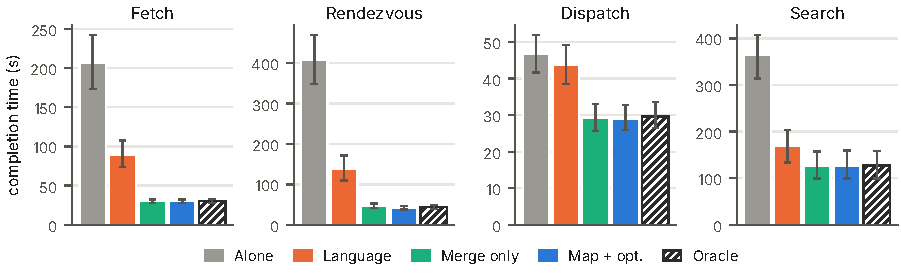
\includegraphics[width=\textwidth]{time_by_task.pdf}
\caption{\textbf{Completion time} by task and condition (mean and 95\% bootstrap interval, 90 episodes per bar). Inventory is omitted because sharing conditions answer it without driving.}
\label{fig:time}
\end{figure*}

\subsection{Words say where to look; a map says where to go}\label{sec:main}
Table~\ref{tab:main} and Fig.~\ref{fig:time} summarize the main grid.
Language alone is a large improvement over working alone.
On the same episodes, it cuts mean completion time by 57\% on fetch (95\% interval 46--66\%), 66\% on rendezvous (58--73\%), and 54\% on search (42--63\%).
The messages cost 643 bytes per episode on average.

The verified, optimized map cuts the time much further: by another 67\% on fetch (60--72\%) and 70\% on rendezvous (62--76\%) relative to \cond{Language}, and by 33\% and 25\% on dispatch and search.
Against working alone, fetch becomes 6.9 times faster and rendezvous 9.7 times faster, and the mean distance driven per episode, over all tasks, falls from 160\,m to 43\,m (61\,m with language).

Fig.~\ref{fig:qual} shows why.
Robot~1 is asked for the white hospital bed in Room~104, which it has never seen.
Alone, it searches the wing for 819\,s.
With language, a teammate replies ``I saw a white hospital bed in the Room~104,'' so Robot~1 drives there and scans the room until it sees the bed itself: 74\,s.
With the map, Robot~1 already knows where the bed is and drives straight to it: 23\,s.
A room name narrows the search to one room; a map position removes the search.

\begin{figure*}[t]
\centering
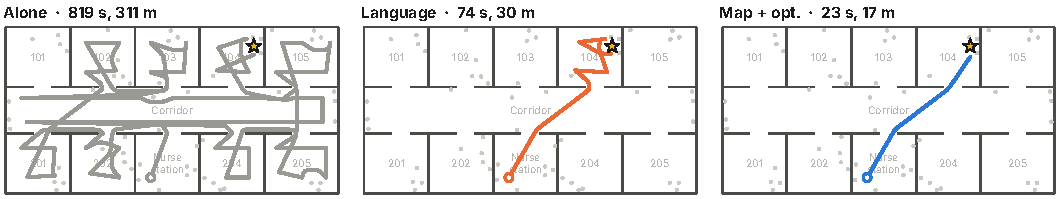
\includegraphics[width=\textwidth]{qual.pdf}
\caption{\textbf{One fetch episode, three media} (hospital, eight robots). Robot~1 must reach the white hospital bed in Room~104 (star), which only a teammate has seen. Lines show Robot~1's path from its start (circle). \emph{Alone}, it searches the wing. \emph{Language}: a teammate names the room, and Robot~1 scans it until it sees the bed. \emph{Map}: the merged map gives the bed's position.}
\label{fig:qual}
\end{figure*}

\subsection{A description must be re-grounded; a map hands over the object}\label{sec:reliab}
Language makes the team faster but not more reliable.
Fetch succeeds in 76\% of episodes with language and 82\% alone; rendezvous in 64\% and 68\%.
The intervals overlap, so language is no more reliable than working alone.
The failures share a cause.
With language, as when working alone, Robot~1 must find the target with its own perception and decide which object matches the description.
Of the 22 failed language fetches, 11 ended at a different object that also fits the description and 7 never found the target. In one hospital episode, a teammate's drifted map put the requested bed in the neighboring look-alike room, and Robot~1 went to the bed there.
Working alone fails in the same two ways (9 and 5 of 16 failures).
A merged map does not have this problem: the teammate's identification, built from its own repeated views, arrives with the object's position.
\cond{Map + opt.} fails only 4 of 90 fetches and 2 of 90 rendezvous episodes.

\subsection{Where talking is enough}\label{sec:counting}
Counting and covering are different.
For inventory, a room-level answer is all the task needs, and \cond{Language} is right in every room in 96\% of episodes, against 90\% for \cond{Map + opt.}
For dispatch, \cond{Language} succeeds in 93\% of episodes against 84\%, although the map finishes in 29\,s instead of 44\,s.
The map's residual errors occasionally leave two copies of one object unmerged, which produces double counts and wasted visits; a room-level count does not have that failure.
Two caveats apply.
Our prior shift gives each room to exactly one robot, so taking the largest count reported for each room is nearly ideal.
If the asker instead sums the reports, inventory accuracy drops to 68\% and dispatch takes twice as long (86\,s), because robots search rooms for instances that were counted twice.

\subsection{Optimization makes the merged map trustworthy}\label{sec:opt}
\cond{Map (merge only)} is as fast as \cond{Map + opt.} but fails more often on every task: 80\% versus 96\% on fetch, 70\% versus 90\% on inventory, 66\% versus 84\% on dispatch, and 86\% versus 96\% on search.
Without the distributed solve, the error of the position Robot~1 drives to is 0.77\,m on fetch, against 0.26\,m with it.
That is enough to stop short of the object or to leave duplicates of the same object in the map.
On inventory and dispatch, merging without optimization is less reliable than not sharing at all (70\% and 66\% versus 94\%).
With optimization the map comes within two points of the oracle on fetch and rendezvous, four on search, and eight on inventory and dispatch, at the same speed.

\begin{table}[t]
\centering
\caption{\textbf{Merge safeguards} by team size, over all tasks and buildings (150 episodes per cell). A wrong merge is any wrong object link or wrong frame alignment, scored against ground truth.}
\label{tab:verify}
\setlength{\tabcolsep}{3.5pt}
\begin{tabular}{lrrrr}
\toprule
Merge & wrong & wrong & robots & \\
& frames & links & joined & score \\
\midrule
\multicolumn{5}{l}{\emph{Look-alike scenes}} \\
\quad Map + opt. & 0.0\% & 1.1\% & 100\% & 89 \\
\quad Verified, no meetings & 7.1\% & 10.9\% & 28\% & 64 \\
\quad No verification & 72.9\% & 43.0\% & 74\% & 45 \\
\multicolumn{5}{l}{\emph{Other scenes}} \\
\quad Map + opt. & 0.0\% & 0.0\% & 100\% & 96 \\
\quad Verified, no meetings & 6.0\% & 0.0\% & 34\% & 59 \\
\quad No verification & 82.0\% & 16.6\% & 86\% & 40 \\
\bottomrule
\end{tabular}

\end{table}

\subsection{Checks and meetings keep the map honest}\label{sec:verify}
Table~\ref{tab:verify} compares the full merge (alignment and link checks plus robot meetings) with the two ablations.
Without checks or meetings, appearance and RANSAC link the maps of most robots, but wrongly: 69\% of four-robot episodes and 78\% of eight-robot episodes contain a wrong merge, and success falls to about a third, below working alone.
With two robots, unchecked matching still works most of the time (17\% wrong merges, 80\% success), because there are fewer maps to confuse.
Keeping the checks but ignoring meetings produces fewer wrong merges (7\% and 14\%), but most alignments are then rejected as ambiguous: only 40\% of robots join at four robots and 26\% at eight, and success drops to about 40\%.
Meetings supply unambiguous frame links, and the checks keep object matches from undoing them.
Together they join every robot with wrong merges in at most 3\% of episodes.

\begin{figure}[t]
\centering
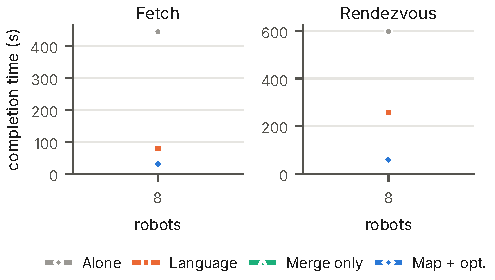
\includegraphics[width=\columnwidth]{scaling.pdf}
\caption{\textbf{Team size} (rendezvous in the office and the hospital, six episodes per point). With a shared map, meeting time grows slowly with team size; alone and with language, robots spend longer searching and more of them fail to arrive. Alone and \cond{Language} overlap at 8 and 10 robots in the right panel.}
\label{fig:scaling}
\end{figure}

\subsection{Team size and cost}\label{sec:cost}
Fig.~\ref{fig:scaling} varies the team size from 1 to 10 for rendezvous.
The time for all robots to meet grows from 158 to 686\,s alone, from 65 to 526\,s with language, and from 31 to 113\,s with the optimized map.
With ten robots, all of them arrive in a third of episodes alone or with language, half with the unoptimized map, 83\% with the optimized map, and every time with the oracle map.
These points rest on six episodes each and should be read as trends.

The map is not free.
\cond{Map + opt.} sends 405\,kB per episode on average: 310\,kB of object descriptors and 95\,kB of separator estimates during optimization.
That is about 630 times the 643 bytes of language messages, or about nine compressed camera images of 45\,kB each.
For robots on a shared wireless network this is small, but under the tight links that motivate distributed SLAM~\cite{choudhary2017ijrr,cieslewski2018icra}, a team may prefer to talk for counting tasks and send the map only when it needs positions.

%% =====================================================================
\section{Limitations}\label{sec:limits}

\textbf{Simulated perception.}
Our descriptors are synthetic.
Real mask-plus-CLIP features are noisier, confuse more categories, and drift with viewpoint and lighting, so real data would produce more look-alike matches.
This would likely widen the gap between verified and unverified merging, but we have not shown it.
Multi-robot open-vocabulary mappers on real sensors~\cite{chang2023hydramulti,gu2025mrcographs,tian2022kimeramulti} are the natural back-end for a real deployment.

\textbf{Placing maps with ground truth.}
We place each map in the floor plan with a rigid fit to the true trajectory (Sec.~\ref{sec:merge}).
This affects every condition equally, but it makes position errors optimistic and gives \cond{Alone} and \cond{Language} correct room names for free.
A real system would localize against the floor plan and would see larger errors, which would likely make room names less reliable and favor the map further.

\textbf{Scripted policies instead of LLMs.}
We isolate the medium by using fixed policies.
Real LLM agents make planning errors, and their errors may differ by medium.
A structured map may be easier for a small model to use correctly than a set of free-form replies, as CoELA's observations of redundant messages suggest~\cite{zhang2024coela}, or a long object list may overflow a small model's context.
Measuring that interaction with the in-browser agents is the next step.

\textbf{A generous, but limited, language channel.}
Our messages carry object names and rooms, not metric descriptions such as ``two meters left of the door.''
Agents could describe positions relative to landmarks, which would close part of the gap at the cost of longer, more ambiguous messages.
Conversely, our channel is lossless and instant, which favors language.

\textbf{Scale and realism.}
The buildings are small and two-dimensional, and the robots are homogeneous.
Idle robots parked at the dock occasionally block a doorway; we count such stalled legs as failures, and they affect at most 6\% of the episodes in any task and condition.
The map's advantage should grow with building size, since the cost of searching a room grows while the cost of driving to a known point does not, but larger and multi-floor buildings remain to be tested.

%% =====================================================================
\section{Conclusion}\label{sec:conclusion}

Should a team of language-model robots talk or share a map?
In our testbed, the answer depends on what the task needs to know.
For ``which room,'' a few hundred bytes of language are enough: messages make search two to three times faster and count objects at least as well as a map does.
For ``which object, and where,'' words fall short, because the robot that hears them must re-find and re-identify the object.
A merged object map hands over both the identity and the position, and makes fetch and rendezvous seven to ten times faster with near-oracle success.
That map is only worth sending if it is built carefully: without distributed optimization or without checks against look-alike places, it can be worse than not sharing.
A practical team might therefore do both: talk by default, and exchange and optimize the map when a task needs positions.
Testing this with real language-model agents, real perception, and larger buildings is the next step.

The code, the experiment harness, and the per-episode results are available at \url{https://itzsid.github.io/hivemap/}, where the simulation and its agents run in the browser.

\bibliographystyle{IEEEtran}
\bibliography{refs}

\end{document}
